%-----------------------------------------------------------------
%	THE PROBLEM
%	!TEX root = ./../main.tex
%-----------------------------------------------------------------
\section{The Problem}

\subsection{Introduction}
Backing up a car can sometimes be a stressful experience. When you have something attached to your car, it gets even more nerve-racking. The problem is that the motion control while moving forward is stable, while reversing the motion is unstable. We want to analyse and solve this problem using mathematical and physical concepts.

To tackle this problem, we need to create a model of the system using differential equations and then design a controller for the system, that is, a mathematical model that can modify dynamically the behaviour of the system to follow a control or reference trajectory.

\begin{figure}[H]
    \centering
    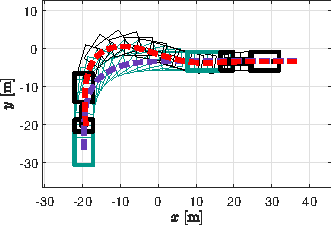
\includegraphics[width=0.55\textwidth]{images/trailer-diagram2}
    \caption{Traversed paths by the car (red line) and the trailer (purple line)}
    \label{fig:trailer-diagram2}
\end{figure}

In short, using figure \ref{fig:trailer-diagram2} as a reference, we would like to predict and control the trajectory purple dashed line (trajectory of the trailer) whilst only having direct access to the physical system that controls the red line (trajectory of the car).

%-----------------------------------------------------------------
\subsection{Modelling the Kinematics}\label{sec:kinematics}
\label{kinem}
Before thinking on the model, we need to make some initial assumptions to simplify the problem. These are the initial assumptions we thought they will ease the modelling work: 
% \begin{itemize}
%     \item The system has a unique pivoting point: the hitch.
%     \item The ground is flat.
%     \item The system is slip free.
%     \item The car backs at constant velocity.
%     \item The trailer's mass is uniformly distributed.
%     \item The trailer has a single-axle.
% \end{itemize}

\begin{itemize}
    \item The system has a unique pivoting point, the hitch. This is completely necessary because it is the responsible of yielding this unstable equilibrium point when driving backwards. 
    \item We assume a flat, nonslippery ground. 
    \item The velocity of the car will be constant when going backwards. Given a steering angle, the car follows a
    circular path.
    \item As we want to work with a geometric model, we need the effect of the mass distribution to be negligible, so we assume a trailer with a uniformly distributed mass. 
    \item Finally, we will work with a trailer that only has a single axle for the wheels.
\end{itemize}

Considering these assumptions, we can focus on the model. We chose a geometric model which only looks at the rate at which the $\phi$ angle changes along time. So our main goal is to predict the $\phi$ angle along the trajectory of the car. 

Figure \ref{fig:geom-model} shows the model of the vehicle-trailer system, and the parameters of the model are presented in table \ref{tab:parameters} below.
\begin{figure}[H]
    \centering
    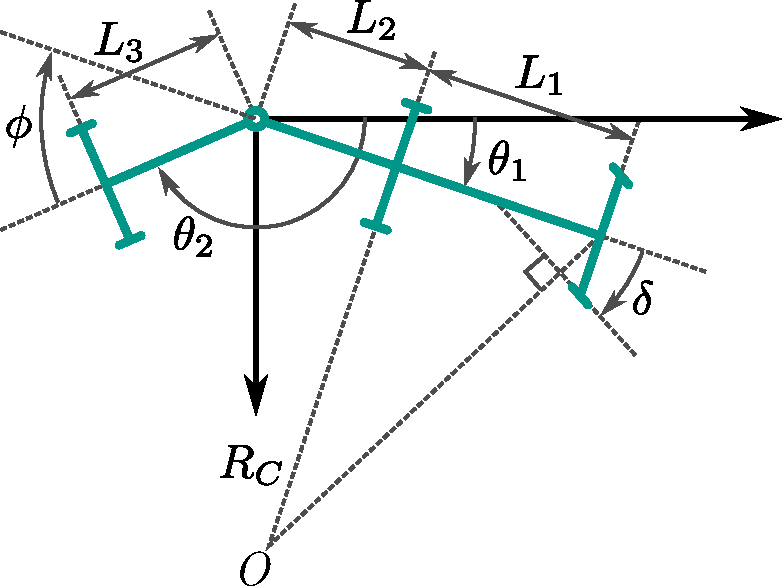
\includegraphics[width=0.5\textwidth]{images/trailer-diagram}
    \caption{Geometric model of the car-trailer system}
    \label{fig:geom-model}
\end{figure}

\begin{table}[H]
    \centering
    \begin{tabularx}{0.95\textwidth}{c X}
        \toprule
        \toprule
        System parameters & Description \\
        \midrule
        $\theta_{1}$  & The angle the car is travelling at with respect to a global coordinate system. \\
        $\theta_{2}$  & The angle the trailer is travelling at with respect to a global coordinate system. \\
        $\phi$        & The angle between the car and the trailer. \\
        $\delta$      & The steering angle of the vehicle's wheels. \\
        $V$           & Reversing speed of the car. \\
        $V_{trailer}$ & Reversing speed of the trailer. \\
        $R_{C}$       & Distance from the centre of rotation $O$ to the rear axle of the car. \\
        $L_{1}$       & Wheelbase of the car. \\
        $L_{2}$       & Overhang from the rear axle of the car to the hitch point. \\ 
        $L_{3}$       & Distance from the trailer axle to the hitch. \\ 
        \bottomrule
    \end{tabularx}
    \caption{Physical parameters of the system described by our model}
    \label{tab:parameters}
\end{table}

If we know $\phi$, we will be able to predict the trajectory of the trailer. The angle $\phi$ is defined as
\begin{align}
    \phi = \pi - (\theta_{2} - \theta_{1}) ,
\end{align}
where $\theta_{2}$ and $\theta_{1}$ are the angles belonging to the car and to the trailer, expressed according to one reference axle. 

Taking the derivative of the angle $\phi$, we obtain
\begin{align}\label{eq:dphi}
    \dot{\phi} = -\dot{\theta}_{2} + \dot{\theta}_{1} ,
\end{align}

Using the distance to the centre of rotation $O$ from the cars' rear axis, an expression for the angular velocity of the car is obtained:
\begin{align}\label{eq:dtheta1-0}
    \dot{\theta}_{1} = -\frac{V}{R_{C}} .
\end{align}
This is, of course, because given a $\delta$, the car follows a uniform circular path. This is what is usually known as Ackerman kinematics (see \cite{steering}), which state that, for a given $\delta$,
every point of the car follows a concentric circular path. The 
centre of these circles can be computed using trigonometry.\\

Using Ackerman kinematics, we can compute the angular velocity as the ratio of the longitudinal speed and the
radius of the path. We can compute the radius of the path using trigonometry, and we obtain:
\begin{align*}
    R_C = \frac{\tan \delta}{L_1}
\end{align*}

Joining the two last expressions we can obtain the following expression:
\begin{align}\label{eq:dtheta1}
    \dot{\theta}_{1} = -\frac{V}{L_{1}} \tan \delta . \tag{\ref{eq:dtheta1-0} bis}
\end{align}

%It is the rate of change of $\theta_{1}$ along time and it depends on the velocity of the car, $V$, the distance between both wheel axles of the car, $L_{1}$, and the angle of the front wheels, $\delta$.

To predict $\phi$, we also need to know how $\theta_{2}$ varies along time. For this reason, we need to know which is the longitudinal speed and the normal speed at the point that joins the car and the trailer. Of course, the longitudinal speed is $V$, and, as the car is rotating at angular velocity $\dot{\theta}_{1}$, the normal speed of that point is $L_2\cdot\dot{\theta}_{1}$. We can compute the longitudinal speed of the trailer by projecting in the longitudinal axis of the trailer the normal and longitudinal speed of the car in the point than joins them:
\begin{align}
    V_{trailer} = -L_{2} \dot{\theta}_{1} \sin \phi + V \cos \phi .
\end{align}
We can also compute the normal speed by projecting the longitudinal and normal speeds in the normal direction of the trailer. This normal speed will be $L_3\dot{\theta_2}$. 
Using this, $\dot{\theta}_{2}$ can be isolated:
\begin{align}\label{eq:dtheta2}
    \dot{\theta}_{2} =  \frac{L_{2} \dot{\theta}_{1} \cos \phi + V \sin \phi }{L_{3}} .
\end{align}

Replacing \eqref{eq:dtheta1} and \eqref{eq:dtheta2} into \eqref{eq:dphi}, we get the variation of $\phi$ along time. It is expressed in terms of the velocity of the car, the distance between the hitch and the trailer axle, the distance between the rear car axle and its hitch, the distance between both wheel axles for the car and the angle of the car’s front wheels:
\begin{align}\label{eq:dotphi-final}
    \dot{\phi} = - \frac{V}{L_{3}} \sin \phi - \frac{V}{L_{1}} \tan \delta \qty( 1 + \frac{L_{2}}{L_{3}} \cos \phi ) .
\end{align}
Of course, this system assumes that $V>0$ when the car is going backwards. As all the geometric arguments are valid, if we take $V < 0$, we will obtain the dynamics of the trailer when the car is going forward.

Here we observe that if we set $\delta = 0$, then the differential equation becomes
\begin{align}\label{eq:dotphi-final-bis}
    \dot{\phi} = - \frac{V}{L_{3}} \sin \phi . \tag{\ref{eq:dotphi-final} bis}
\end{align}

In this case, $\phi = 0$ is a critical point of the differential equation. To analyse its stability, we have to discuss the sign of:
\begin{align}\label{eq:stability-0}
    \dv{\phi} \qty( - \frac{V}{L_{3}} \sin \phi )  = - \frac{V}{L_{3}} \cos \phi
\end{align}
at the critical point. At $\phi = 0$, the previous expression becomes
\begin{align}\label{eq:stability}
    -\frac{V}{L_3} . \tag{\ref{eq:stability-0} bis}
\end{align}
This shows that when $V > 0$ (car going backwards) this critical point is unstable, and when $V < 0$ the point is stable.

\bigskip
In the simulation, we will also take into account the phenomenon of jackknifing. A trailer jackknifes when its $\phi$
angle grows up to the point where the trailer contacts the car.
Of course, by all means we want to avoid this situation. As a general fact accepted in the bibliography, (see \cite{jack}) when $\phi$ surpasses a critical $\phi_{crit}$, the trailer cannot be controlled and the jackknifing phenomenon occurs.

\bigskip
We have already derived a model for the kinematics of the trailer with respect to the movement of the car. In order to produce a proper simulation of the whole system, we need to model the kinematics of the car as well. The model that we have used is based on Ackerman kinematics. The result of the model is that every point of the car moves through a circular path of centre $O$ (see Figure \ref{fig:geom-model}).


%-----------------------------------------------------------------
\subsection{Controller Design}

We think that our problem is mainly a control theory based problem. The aim is to design a controller for the system to drive the state $\phi$ to the wished state by changing the steering angle $\delta$. We would like to consider a linear controller which applies to the nonlinear model. The following section gives a mathematical introduction on control theory and afterwards the controller is presented.
